\documentclass[a4paper,11.5pt]{article} % тип документа


%%%Библиотеки
%\usepackage[warn]{mathtext}
%\usepackage[T2A]{fontenc} % кодировка
\usepackage[utf8]{inputenc} % кодировка исходного текста
\usepackage[english,russian]{babel} % локализация и переносы
\usepackage{caption}
\usepackage{listings}
\usepackage{amsmath,amsfonts,amssymb,amsthm,mathtools}
\usepackage{wasysym}
\usepackage{graphicx}%Вставка картинок правильная
\usepackage{float}%"Плавающие" картинки
\usepackage{wrapfig}%Обтекание фигур (таблиц, картинок и прочего)
\usepackage{fancyhdr} %загрузим пакет
\usepackage{lscape}
\usepackage{xcolor}
\usepackage[normalem]{ulem}
\usepackage{hyperref}

%%%Конец библиотек




%%%Настройка ссылок
\hypersetup
{
colorlinks=true,
linkcolor=blue,
filecolor=magenta,
urlcolor=blue
}
%%%Конец настройки ссылок


%%%Настройка колонтитулы
\pagestyle{fancy}
\fancyhead{}
\fancyhead[L]{Лаб. работа 2.2.1}
\fancyhead[R]{Талашкевич Даниил, группа Б01-009}
\fancyfoot[C]{\thepage}
%%%конец настройки колонтитулы



\begin{document}
%%%%Начало документа%%%%


%%%Начало титульника
\begin{titlepage}

\newpage
\begin{center}
\normalsize Московский физико-технический институт \\(госудраственный университет)
\end{center}

\vspace{6em}

\begin{center}
\Large Лабораторная работа по термодинамике\\
\end{center}

\vspace{1em}

\begin{center}
\large \textbf{Исследование взаимной диффузии газов [2.2.1]}
\end{center}

\vspace{2em}

\begin{center}
\large Талашкевич Даниил Александрович\\
Группа Б01-009
\end{center}

\vspace{\fill}

\begin{center}
Долгопрудный \\19.04.2021
\end{center}

\end{titlepage}
%%%Конец Титульника



%%%Настройка оглавления и нумерации страниц
\thispagestyle{empty}
\newpage
\tableofcontents
\newpage
\setcounter{page}{1}
%%%Настройка оглавления и нумерации страниц


%%%%%%Начало работы с текстом%%%%%%
\section{Аннотация}
\subsection{Цель работы}

\textbf{Цель работы:} 1) регистрация зависимости концентрации гелия в воздухе от времени с помощью датчиков теплопроводности при разных начальных давлениях смеси газов; 2) определение коэффициента диффузии по результатам измерений.

\subsection{Используемое оборудование}

\textbf{В работе используются:} измерительная установка; форвакуумный насос; баллон с газом (гелий); манометр; источник питания;
магазин сопротивлений; гальванометр; секундомер.

\subsection{Теоретическое введение}

Диффузией называют самопроизвольное взаимное проникновение веществ друг в друга, происходящее вследствие хаотичного теплового движения молекул. При перемешивании молекул разного сорта говорят о взаимной (или концентрационной) диффузии. Диффузия в системе, состоящей из двух компонентов $a$ и $b$ (бинарная смесь), подчиняется закону Фика: плотности потока компонентов $j_{a, b}$ (количество частиц, пересекающих единичную площадку в единицу времени) пропорциональны градиентам их концентраций $\nabla n_{a, b}$, что в одномерном случае можно записать как 
\begin{equation}
	j_a = -D \dfrac{\partial n_a}{\partial x},~j_b = -D \dfrac{\partial n_b}{\partial x},
\end{equation}
где $D$ -- коэффициент взаимной диффузии компонентов. Знак «минус» отражает тот факт, что диффузия идёт в направлении выравнивания концентраций. Равновесие достигается при равномерном распределении вещества по объёму сосуда ($\dfrac{\partial n}{\partial x} = 0$).

В данной работе исследуется взаимная диффузия гелия и воздуха. Давление $P$ и температура $T$ в условиях опыта предполагаются неизменными: 

$P = (n_{He} + n_{\text{в}}) k_{\text{Б}} T = const$, где $n_{He}$ и $n_{\text{в}}$ --— концентрации (объёмные плотности) диффундирующих газов. Поэтому для любых изменений концентраций справедливо $\Delta n_{\text{в}} = - \Delta n_{He}$. Следовательно, достаточно ограничиться описанием диффузии одного из компонентов, например гелия 
\begin{equation}
	n_{He}:j_{He} = -D \dfrac{\partial n_{He}}{\partial x}
\end{equation}

Приведём теоретическую оценку для коэффициента диффузии. В работе концентрация гелия, как правило, мала ($n_{He} \ll n_{\text{в}}$). Кроме того, атомы гелия существенно легче молекул, составляющих воздух ($\mu_{He} \ll \mu_{N_2}, \mu_{O_2}$), значит и их средняя тепловая скорость велика по сравнению с остальными частицами. Поэтому перемешивание газов в работе можно приближенно описывать как диффузию примеси лёгких частиц $He$ на практически стационарном фоне воздуха. Коэффициент диффузии в таком приближении равен 
\begin{equation}
	D = \dfrac{1}{3} \lambda \overline{v},
\end{equation}
где $\overline{v} = \sqrt{\dfrac{8RT}{\pi \mu}}$ -- средняя тепловая скорость частиц примеси,
$\lambda = \dfrac{1}{n_0 \sigma}$ -- их длина свободного пробега, $n_0$ -- концентрация рассеивающих центров (фона), $\sigma$ -- сечение столкновения частиц примеси с частицами фона.

В общем случае необходимо учитывать диффузию каждого из компонентов. Более подробное рассмотрение показывает, что для бинарной смеси формула $(2)$ сохраняется, если $1)$ под $\lambda$ понимать величину $\lambda = \dfrac{1}{n_{\sum} \cdot \sigma}$, где $n_{\sum} = n_{He} + n_{\text{в}} = \dfrac{P}{k_{\text{Б}} T}$ -- полная концентрация частиц, и $2)$ под $\overline{v}$ понимать среднюю относительную скорость частиц разных сортов. Для бинарной смеси, как в нашем случае, $\overline{v} = \sqrt{\dfrac{8 k_{\text{Б}} T}{\pi \overline{m}}}$, где $\overline{m}$ -- приведённая масса частиц смеси.

Таким образом, теория предсказывает, что коэффициент диффузии бинарной смеси обратно пропорционален давлению в системе $D \propto \dfrac{1}{P}$, и не зависит от пропорций компонентов, что и предлагается проверить в работе экспериментально.

\section{Экспериментальная установка}

Для исследования взаимной диффузии газов и измерения коэффициента взаимной диффузии $D$ используется два сосуда объёмами $V_1$ и $V_2$ ($V_1 \approx V_2 \equiv V$), соединенные трубкой длины $L$ и сечения $S$ (рис. 1). Предполагается, что сосуды заполнены смесью двух газов при одинаковом давлении, но с различной концентрацией компонентов. Вследствие взаимной диффузии, проходящей в соединительной трубке, концентрации компонентов в сосудах с течением времени выравниваются.

\begin{wrapfigure}[16]{l}{0.23 \linewidth} 
    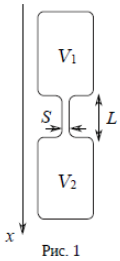
\includegraphics{2211.png}
\end{wrapfigure}

Важно отметить, что диффузия -- относительно медленный процесс, и для его наблюдения необходимо отсутствие конвекции, т. е. макроскопических течений газа. Для этого необходимо обеспечить равенство давлений и температур в сосудах до начала измерений.

В общем случае концентрации компонентов $n(t, x)$ зависят как от координаты, так и от времени. Задача упрощается, если объём соединительной трубки мал по сравнению с объёмами сосудов -- тогда концентрации газов $n_1(t)$ и $n_2(t)$ внутри каждого сосуда можно считать постоянными по всему объёму сосуда, и принять, что процесс выравнивания концентраций происходит благодаря диффузии в трубке.

Рассмотрим подзадачу о диффузии в соединительной трубке. Предположим сперва, что концентрации примеси (гелия) на её торцах поддерживаются постоянными и равными $n_1$ и $n_2$ соответственно. Тогда через некоторое время (оценку этого времени см. ниже ф-лу $(9)$) в трубке установится стационарный поток частиц, одинаковый в каждом сечении трубки (в противном случае, если бы поток зависел от $x$, частицы бы накапливались в трубке, и процесс перестал бы быть стационарным). Применяя закон Фика в трубке, получим $$j = -D \dfrac{\partial n}{\partial x} = const.$$
Следовательно, распределение концентрации в трубке $n(x)$ -- линейная функция:
\begin{equation}
	n(x) = \dfrac{\Delta n}{L} x
\end{equation}
и плотность потока частиц всюду постоянна и равна
\begin{equation}
	j = -D \dfrac{\Delta n}{L},
\end{equation}
где $\Delta n = n_2 - n_1$ -- разность концентраций гелия на концах трубки.

Теперь вернёмся к процессу выравнивания концентраций в сосудах. Частицы перетекают из сосуда $2$ в сосуд $1$ по трубке и концентрации $n_1(t)$ и $n_2(t)$ меняются во времени. Предположим, что этот процесс происходит достаточно медленно, так что в трубке в любой момент времени успевает установиться практически стационарное течение, описываемое формулами $(4)$, $(5)$. Такое приближение называют квазистационарным. Кроме того, будем считать, что в пределах каждого сосуда частицы распределены равномерно, так что концентрации примеси вблизи трубки и в остальных частях сосуда отличаются мало. Тогда полное число частиц примеси в сосудах равно соответственно $N_1 = n_1 V$ и $N_2 = n_2 V$. Произведение плотности потока $(5)$ на площадь сечения трубки $S$ даёт количество частиц, пересекающих в единицу времени любое поперечное сечение трубки. Поэтому
\begin{equation}
	\dfrac{dN_1}{dt} = jS, ~\dfrac{dN_2}{dt} = -jS.
\end{equation}
Выразим отсюда скорость изменения $\Delta n$. Вычитая из второго равенства первое и деля результат на объём сосуда $V$, с учетом $(4)$ получим
\begin{equation}
	\dfrac{d(\Delta n)}{dt} = - \dfrac{\Delta n}{\tau},
\end{equation}
где введено обозначение
\begin{equation}
	\tau = \dfrac{1}{D} \dfrac{VL}{2S}.
\end{equation}
Интегрируя $(6)$, получаем, что разность концентраций будет убывать по экспоненциальному закону
\begin{equation}
	\Delta n = \Delta n_0 e^{-t/\tau},
\end{equation}
где $\Delta n_0$ --— разность концентраций примеси в сосудах в начальный момент времени. Видно, что величина $\tau$ есть характерное время выравнивания концентраций между сосудами. Оно определяется геометрическими размерами установки и коэффициентом диффузии.

Отметим, что для применимости квазистационарного приближения необходимо убедиться, что время процесса $\tau$ много больше характерного времени диффузии отдельной частицы вдоль трубки $L$, которое согласно закону Эйнштейна–Смолуховского по порядку величины равно
\begin{equation}
	\tau_{\text{диф}} \sim \dfrac{L^2}{2D}.
\end{equation}
Таким образом, необходимо выполнение неравенства $\tau \gg \tau_{\text{диф}}$, что с учётом $(8)$ и $(10)$ может быть переписано как $SL \ll V$, то есть объём трубки должен быть много меньше объёма сосудов.

Кроме того, если сосуды расположены вертикально, может возникнуть вопрос о влиянии силы тяжести на диффузию. Влиянием гравитации можно пренебречь, если перепад потенциальной энергии в сосуде много меньше энергии теплового движения частиц $mgh \ll k_{\text{Б}} T$. Нетрудно проверить, что для молекулярной диффузии в нашем эксперименте это выполняется с большим запасом.

\section{Методика измерений}

 Для измерения разности концентраций в установке применяются датчики теплопроводности. При этом используется тот факт, что теплопроводность смеси зависит от её состава. В общем случае зависимость $\kappa(n)$ довольно сложна, однако при малой разности $\Delta n$ концентраций в сосудах можно ожидать, что разность теплопроводностей будет изменяться прямо пропорционально $\Delta n$: $$\Delta \kappa = \kappa (n_2) - \kappa (n_1) \approx const \cdot \Delta n.$$
Эксперименты показывают, что если доля примеси гелия составляет менее $15\%$, отклонение от линейной зависимости не превышает $0,5\%$, что для наших целей вполне достаточно.

Сами датчики теплопроводности устроены следующим образом. Тонкая платиновая проволочка, протянутая вдоль оси стеклянного цилиндра, нагревается током. Внутренняя полость датчика сообщается с объёмом камеры через отверстия, размеры которых таковы, что скорость диффузии из объёма сосуда в полость датчика значительно больше скорости диффузии из одного объёма в другой. Таким образом, состав газа в датчике практически совпадает с составом газа в объёме. Тепло от проволочки к стенке цилиндра передаётся главным образом за счёт теплопроводности газа, находящегося внутри цилиндра. При заданной мощности нагревания приращение температуры проволочки и, следовательно, приращение её сопротивления пропорциональны теплопроводности газа.

Для измерения сопротивлений используется мостовая схема, позволяющая определять разность показаний датчиков с высокой точностью. Мост балансируется при заполнении сосудов (и датчиков) одной и той же смесью. При заполнении сосудов смесями различного состава возникает «разбаланc» моста. При незначительном различии в составах смесей показания вольтметра, подсоединённого к диагонали моста, будут пропорциональны разности концентраций примеси: $U \propto \Delta \kappa \propto \Delta n$. В процессе диффузии разность концентраций убывает по закону $(8)$, и значит по тому же закону изменяется напряжение: 
\begin{equation}
	U = U_0 e^{-t/\tau},
\end{equation}
где $U_0$ --- показание гальванометра в начальный момент времени. Измеряя экспериментально зависимость $U(t)$, можно получить характерное время процесса $\tau$, откуда по формуле $(8)$ определить коэффициент диффузии $D$.
\begin{center}
    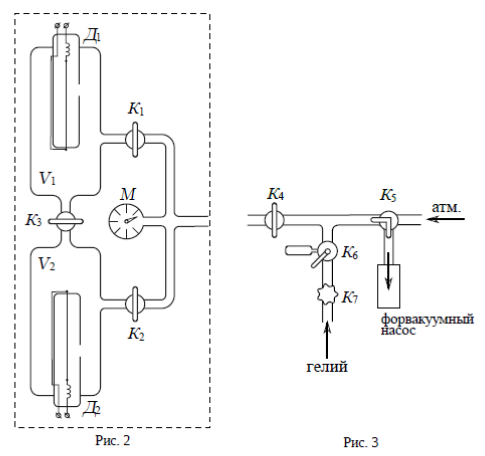
\includegraphics[scale = 0.67]{2212.png}
\end{center}

\section{Экспериментальная установка}

Схема измерительной части установки приведена на рис. 2. Она соединена с системой откачки и напуска воздуха и гелия. Для откачки используется форвакуумный насос. Конструкции системы откачки и напуска могут быть различны в зависимости от установки (схемы и описания см. на столах); один из вариантов изображен на рис. 3. Часть установок компьютеризировано, что позволяет записывать зависимость показаний вольтметра $U(t)$ в реальном времени (на остальных установках фиксация $U(t)$ ведется вручную с помощью секундомера).

Измерительная часть установки состоит из двух сосудов $V_1$ и $V_2$, размещённых вертикально. Краны $K_1$ и $K_2$ служат для управления откачкой и подачей воздуха/гелия в сосуды. Диффузия осуществляется через тонкую короткую трубку, соединяющую сосуды, оснащённую краном $K_3$. К соединительным трубкам подключен манометр $M$, измеряющий разность давлений между соединительными трубками и атмосферой, и позволяющий измерять давления в разных частях системы (в зависимости от положения кранов).

Выравнивание давлений в сосудах $V_1$ и $V_2$ без изменения состава газов в них может быть осуществлено через обводные трубки посредством кратковременного открытия кранов $K_1$ и $K_2$ (при закрытом $K_3$).

Гелий содержится в баллоне (не изображен на рис.) под давлением, превышающим атмосферное. Для предотвращения избыточного расхода гелия и его неконтролируемого проникания в установку предусмотрен металлический кран $K_7$, отделяющий её от баллона с гелием. Его открывают только на время непосредственного заполнения установки гелием, остальное время он должен быть закрыт. Для подачи малых порций гелия предусмотрен двухходовый кран с дозатором (рис. 4). При повороте рычажка $P$ в положение $I$ гелий в небольшом количестве поступает в дозатор (если открыт $K_7$), а при повороте $P$ в положение $II$ порция из дозатора поступает в установку.
\begin{center}
    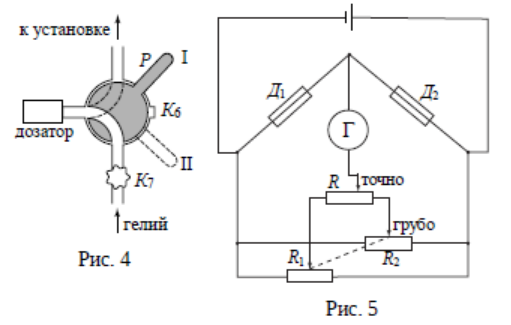
\includegraphics[scale = 1.0]{2213.png}
\end{center}
Датчики теплопроводности $\text{Д}_1$ и $\text{Д}_2$, расположенные в сосудах $V_1$ и $V_2$ соответственно, включены в мостовую электрическую схему согласно рис. 5. В одну из диагоналей моста включён высокочувствительный вольтметр (гальванометр) Г, к другой подключается источник небольшого постоянного напряжения. Сопротивления проволок датчиков составляют одно из плеч моста. Второе плечо составляют переменные сопротивления $R_1$, $R_2$ и $R$, служащие для установки показаний вольтметра Г на нуль (балансировка моста). Сопротивления $R_1$ и $R_2$ спарены (их подвижные контакты находятся на общей оси) и изменяются одновременно при повороте ручки грубой регулировки. Точная балансировка выполняется потенциометром $R$. Балансировку необходимо проводить перед каждым экспериментом заново: при этом установка заполняется чистым газом (воздухом без гелия) при давлении, близком «рабочему» (при котором затем будут проводится измерения).

\newpage

\section{Ход работы}
\subsection{Основная часть работы}

Подготовим установку к работе, сбалансируем измерительный мост при предполагаемом «рабочем» давлении (суммарном давлении смеси в эксперименте $P_{\sum}$). В качестве начального рабочего давления возьмем $P_{\sum} \sim 40$ торр. Затем приготовим рабочие смеси для проведения измерений. В одном из сосудов (например, $V_2$) должен оказаться чистый воздух, в другом ($V_1$) смесь воздуха с гелием. Давления в сосудах должны быть одинаковы и равны рабочему $P_{\sum}$. При этом учтем, что процесс диффузии начнётся после открывания крана $K_3$. Откроем $K_3$ и будем снимать на камеру телефона, как меняются показания вольтметра с течением времени. Измерение продолжим до тех пор, пока напряжение не упадет хотя бы на $30-50\%$. При измерениях снимаем показания каждые $10$ с. 

Проделаем измерения при различных значениях рабочего давления в диапазоне $40-300$ торр (всего $5$ значений). При планировании эксперимента учтем, что с увеличением давления уменьшается коэффициент диффузии, что приводит к пропорциональному увеличению времени наблюдений. При этом учтем, что время отсчитывалось от начала съемки видео, а не от начала открытия крана $K_3$, поэтому время отсчитывается везде от 10 секунд.

Занесем все получившиеся данные в таблицы: % 7.686


\begin{table}[h]
	\caption{Зависимость $U(t)$ при $P_{\sum} = 35 $ торр.}
\begin{tabular}{| c | c | c | c | c | c | c | c | c | c |}
\hline
t, c & 10 & 20 & 30 & 40 & 50 & 60 & 70 & 80 & 90 \\ \hline
U, мB & 15,74 & 14,42 & 13,34 & 12,34 & 11,45 & 10,64 & 9,91 & 9,18 & 8,48 \\ \hline
$ln(U)$ & 2,76 & 2,67 & 2,59 & 2,51 & 2,44 & 2,36 & 2,29 & 2,22 & 2,13 \\ \hline
\end{tabular}\\

	\caption{Зависимость $U(t)$ при $P_{\sum} = 100 $ торр.}
\begin{tabular}{| c | c | c | c | c | c | c | c | c | c |}
\hline
t, c & 10 & 20 & 30 & 40 & 50 & 60 & 70 & 80 & 90  \\ \hline
U, мB & 15,36 & 14,56 & 14,09 & 13,75 & 13,52 & 13,29 & 13,10 & 12,88 & 12,69  \\ \hline
$ln(U)$ & 2,73 & 2,68 & 2,65 & 2,62 & 2,60 & 2,59 & 2,57 & 2,56 & 2,54  \\ \hline
\\  \hline
t, c & 100 & 110 & 120 & 130 & 140 & 150 & 160 &&  \\ \hline
U, мB & 12,49 & 12,30 & 12,08 & 11,45 & 11,24 & 11,02 & 10,81 && \\ \hline
$ln(U)$ & 2,52 & 2,51 & 2,49 & 2,44 & 2,42 & 2,40 & 2,38 && \\ \hline
\end{tabular}\\
\end{table}

\begin{table}
	\caption{Зависимость $U(t)$ при $P_{\sum} = 150 $ торр.}
\begin{tabular}{| c | c | c | c | c | c | c | c | c | c |}
\hline
t, c & 10 & 20 & 30 & 40 & 50 & 60 & 70 & 80 & 90  \\ \hline
U, мB & 15,06 & 14,53 & 14,19 & 13,93 & 13,71 & 13,54 & 13,38 & 13,21 & 12,94  \\ \hline
$ln(U)$ & 2,71 & 2,68 & 2,65 & 2,63 & 2,62 & 2,61 & 2,59 & 2,58 & 2,56  \\ \hline
\\  \hline
t, c & 100 & 110 & 120 & 130 & 140 & 150 & 160 & 170 & 180    \\ \hline
U, мB & 12,84 & 12,70 & 12,49 & 12,28 & 12,08 & 11,88 & 11,67 & 11,48 & 11,28  \\ \hline
$ln(U)$ & 2,55 & 2,54 & 2,52 & 2,51 & 2,49 & 2,47 & 2,46 & 2,44 & 2,42 \\ \hline
\\  \hline
t, c & 190 & 200 &&&&&&&\\ \hline
U, мB & 11,07 & 10,47 &&&&&&&\\ \hline
$ln(U)$  & 2,40 & 2,35 &&&&&&&\\ \hline
\end{tabular}\\

	\caption{Зависимость $U(t)$ при $P_{\sum} = 200 $ торр.}
\begin{tabular}{| c | c | c | c | c | c | c | c | c | c |}
\hline
t, c & 10 & 20 & 30 & 40 & 50 & 60 & 70 & 80 & 90 \\ \hline
U, мB & 15,97 & 15,43 & 15,00 & 14,74 & 14,53 & 14,31 & 14,04 & 13,92 & 13,72  \\ \hline
$ln(U)$ & 2,77 & 2,74 & 2,71 & 2,69 & 2,68 & 2,66 & 2,64 & 2,63 & 2,62   \\ \hline
\\  \hline
t, c & 100 & 110 & 120 & 130 & 140 & 150 & 160 & 170 & 180    \\ \hline
U, мB & 13,55 & 13,37 & 13,16 & 12,98 & 12,77 & 12,55 & 12,34 & 12,15 & 11,92   \\ \hline
$ln(U)$ & 2,61 & 2,59 & 2,58 & 2,56 & 2,55 & 2,53 & 2,51 & 2,50 & 2,48  \\ \hline
\\  \hline
t, c & 190 & 200 & 210 &&&&&&\\ \hline
U, мB & 11,71 & 11,49 & 11,27 &&&&&&\\ \hline
$ln(U)$ & 2,46 & 2,44 & 2,42 &&&&&&\\ \hline
\end{tabular}\\

	\caption{Зависимость $U(t)$ при $P_{\sum} = 250 $ торр.}
\begin{tabular}{| c | c | c | c | c | c | c | c | c | c |}
\hline
t, c & 10 & 20 & 30 & 40 & 50 & 60 & 70 & 80 & 90 \\ \hline
U, мB & 15,25 & 15,02 & 14,84 & 14,68 & 14,62 & 14,40 & 14,27 & 14,16 & 14,03  \\ \hline
$ln(U)$ & 2,72 & 2,71 & 2,70 & 2,69 & 2,68 & 2,67 & 2,66 & 2,65 & 2,64     \\ \hline
\\  \hline
t, c & 100 & 110 & 120 & 130 & 140 & 150 & 160 & 170 & 180    \\ \hline
U, мB & 13,93 & 13,81 & 13,70 & 13,59 & 13,47 & 13,35 & 13,25 & 13,14 & 13,03    \\ \hline
$ln(U)$ & 2,63 & 2,63 & 2,62 & 2,61 & 2,60 & 2,59 & 2,58 & 2,58 & 2,57  \\ \hline
\\  \hline
t, c & 190 & 200 & 210 &&&&&&\\ \hline
U, мB & 12,51 & 12,38 & 13,26 &&&&&&\\ \hline
$ln(U)$  & 2,53 & 2,52 & 2,51 &&&&&&\\ \hline
\end{tabular}\\
\end{table}

\newpage

Построим с помощью программы Matlab график зависимости $U(t)$ при разных $P_{\sum}$ для каждой таблицы соответственно. Графики представлены в конце.

Теперь получим коэффициент взаимной диффузии для каждого $P_{\sum}$. Воспользовавшись формулой $(11)$ имеем: 

$U = U_0 e^{-t/\tau} \Rightarrow \ln U = - \dfrac{1}{\tau} t + \ln U_0 $, где $\tau = \dfrac{1}{D} \dfrac{VL}{2S} \Rightarrow D = \dfrac{VL}{2 \tau S}$,

где $V, L, S$ -- параметры экспериментальной установки. При этом $V = (360 \pm 10)~ \text{см}^3, ~\dfrac{L}{S} = (7,0 \pm 0,1)~ \text{см}^{-1}$. A $ -\dfrac{1}{\tau}$ коэффициент наклона соответсвующего графика. Полученные $D$ занесем в таблицу.

\hspace{1mm}

Таблица 6. Зависимость коэффициента диффузии от обратного давления.
\begin{center}
\begin{tabular}{ | c | c | c | c | c | c | c |}
\hline
$-\dfrac{1}{\tau}$, \text{c}$^{-1}$ & -0,0076 & -0,0021 & -0,0016 & -0,0014 & -0,0010 \\ \hline
$\tau$, c & 131,58 & 476,19 & 625,00 & 714,29 & 1000,00  \\ \hline
D, $\dfrac{\text{см}^2}{c}$ & 9,58 & 2,65 & 2,02 & 1,76 & 1,26 \\ \hline
$P_{\sum},$ торр& 35 & 100 & 150 & 200 & 250  \\ \hline
$\dfrac{1}{P_{\sum}}, \frac{1}{\text{торр}}$ & 0,033 & 0,010 & 0,007 & 0,005 & 0,004 \\ \hline
\end{tabular}
\end{center}

Также построим график зависимости $D\bigg(\dfrac{1}{P_{\sum}}\bigg)$(приведен в конце) и с помощью Мatlab получим уравнение сглаживающей прямой:
\begin{equation}
	y = 286,26\cdot x + 0,0761
\end{equation}
Посчитаем теперь требуемые в задании величины, а именно:\\
	-- коэффициент взаимной диффузии при атмосферном давлении($D(P_{\text{атм}})$) \\
	-- длину свободного пробега атомов гелия($\lambda_{He}$)\\
	-- эффективное сечение столкновений атомов гелия с молекулами воздуха($S_{He}$)\\
	
Коэффициент взаимной диффузии получим экстраполяцией сгдаживающей прямой до атмосферного давления, т.е.
\begin{equation}
	D(P_{\text{атм}}) = \frac{286,26}{760} + 0,0761 = 0,45\ \frac{\text{см}^2}{c}
\end{equation}

Длину свободного пробега посчитаем по формуле:
\begin{equation}
	\lambda_{He} = 3\cdot D(P_{\text{атм}})\cdot \sqrt{\dfrac{\pi \mu}{8RT}} \Rightarrow  \lambda_{He} = 107\ \text{нм}
\end{equation}

Эффективное сечение столкновений атомов гелия с молекулами воздуха посчитаем по формуле:
\begin{equation}
	S_{He} = \frac{kT}{p\lambda} \Rightarrow S_{He} = 3,83 \cdot 10^{-19}\ \text{м}^2
\end{equation}


\subsection{Проверка утверждения о независимости коэффициента взаимной диффузии от пропорций компонентов (*)}

В предыдущих пунктых у нас было соотношение порядка 1 $He$ к 10 Возд, в этом пункте сделаем наоборот, то есть пропорция компонентов изменится аж в 100 раз. Полученные данные представленны в следующей талице (при $P_{\sum}$ = 40 торр, так же в данной таблице представлена лишь часть данных, так как всего вышло 250 точек, что очень много и нет смысла всех их вносить в таблице):

\begin{table}[!h]
	\caption{Зависимость $U(t)$ при $P_{\sum} = 40 $ торр.}
\begin{tabular}{| c | c | c | c | c | c | c | c | c | c |}
\hline
t, c & 10 & 20 & 30 & 40 & 50 & 60 & 70 & 80 & 90  \\ \hline
U, мB & 19,3 & 19,2 & 17,15 & 16,17 & 15,25 & 14,37 & 13,55 & 12,77 & 12,03  \\ \hline
$ln(U)$ & 2,96 & 2,90 & 2,84 & 2,78 & 2,72 & 2,67 & 2,61 & 2,55 & 2,49  \\ \hline
\\  \hline
t, c & 100 & 110 & 120 & 130 & 140 & 150 & 160 & 170 & 180    \\ \hline
U, мB & 11,34 & 10,69 & 10,07 & 9,48 & 8,92 & 8,39 & 7,90 & 7,42 & 6,98  \\ \hline
$ln(U)$ & 2,43 & 2,37 & 2,31 & 2,25 & 2,19 & 2,13 & 2,07 & 2,00 & 1,94 \\ \hline
\end{tabular}\\
\end{table}

Построим график полученных данных, а по ним рассчитаем коэффициент диффузии, затем сравним его с полученными значениями:

\begin{figure}[!h]
	\center{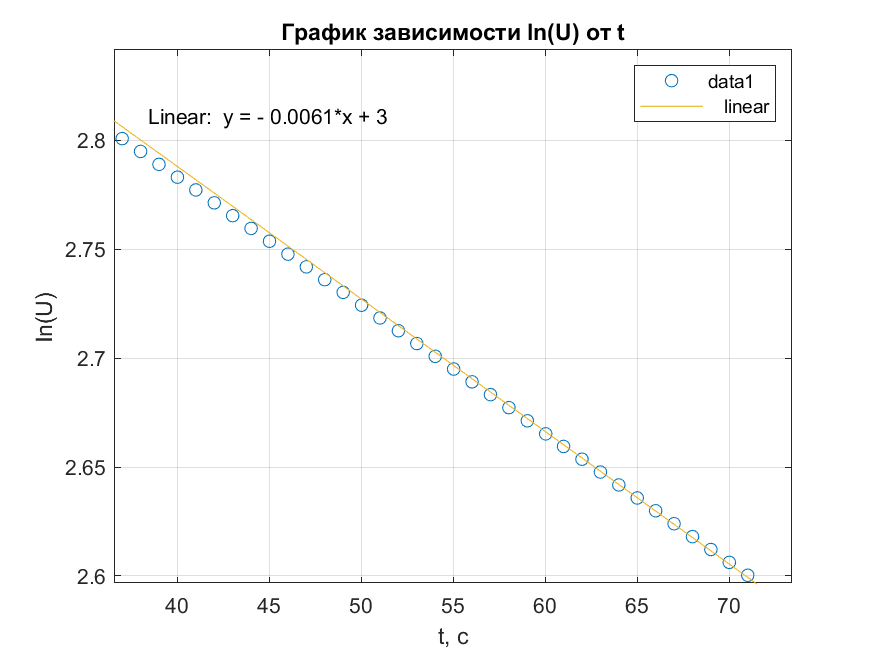
\includegraphics[scale = 0.72]{7_2.png}}
\end{figure}

Полученное значение $D = 14,37 \pm 0,43 \frac{\text{см}^2}{c}.$ И как будет видно позже, это значение не совсем в пределах погрешности ложится на график зависимости $D(\frac{1}{P})$, откуда следует, что утверждения о независимости коэффициента взаимной диффузии от пропорций компонентов не совсем справедливо. Это можно объяснить следующим: это предположение было бы справедливым, если бы молярные массы сильно различались, на порядок много больший, чем 1. У воздуха молярная масса 29, а у гелия, в идеале, 4, однако гелий мог быть с примесями более тяжелых газов, тогда его молярную массу можно посчитать порядка 7 (для оценки). Для того, чтобы понять как зависит коэффициент диффузии от молярных масс я решил соответствующую задачу. В ней видно, что при наших молярных масс как раз таки и видно отклонение.

\subsection{Аппроксимация полученных данных}

Для каждого графика рассчитаем погрешность коэффициента угла наклона прямой $k$ с помощью программы  Matlab с использованием МНК по формуле:
\begin{equation}
	\sigma_k = \dfrac{1}{\sqrt{n}} \sqrt{\dfrac{\langle\ln^2 U\rangle - \langle\ln U\rangle^2}{\langle t^2\rangle - \langle t\rangle^2} - \left(k\right)^2}  
\end{equation}

Тогда следуя из линейность погрешность будет вычисляться вот так:
\begin{equation}
	\sigma_\tau = \dfrac{\sigma_k\cdot \tau}{k}
\end{equation}
Так как $D$ находится по формуле $D = \dfrac{VL}{2 \tau S}$, то его погрешность $\sigma_D$ бужет находится по такой формуле:
\begin{equation}
	\sigma_D = D \cdot \sqrt{\left(\dfrac{\sigma_{\frac{L}{S}}}{\frac{L}{S}}\right)^2 + \left(\dfrac{\sigma_{\tau}}{\tau}\right)^2 + \left(\dfrac{\sigma_V}{V}\right)^2}.
\end{equation}

Тогда относительная погрешность для $D$:
\begin{equation}
	\varepsilon_D = \frac{\sigma_D}{D}\cdot 100\%
\end{equation}

Получив все формулы найдем вычислим с помощью Matlab:
\begin{multline}
	\sigma_{k1} = 0,0002\ c^{-1},~~~\sigma_{k2} = 0,0001\  c^{-1},~~~\sigma_{k3} = 0,0001\ c^{-1},~~~\\
	\sigma_{k4} = 0,0001\ c^{-1},~~~\sigma_{k5} = 0,0002\ c^{-1}~~~
\end{multline}

\begin{multline}
	\sigma_{\tau 1} = 3,46\ c,~~~\sigma_{\tau 2} = 22,68\ c,~~~\sigma_{\tau 3} = 39,06\ c,~~~\\
	\sigma_{\tau 4} = 51,02\ c,~~~\sigma_{\tau 5} = 200,00\ c~~~
\end{multline}

\begin{multline}
	\sigma_{D1} = 0,38\ \frac{\text{см}^2}{c},~~~\sigma_{D2} = 0,15\ \frac{\text{см}^2}{c},~~~\sigma_{D3} = 0,14\ \frac{\text{см}^2}{c},~~~\\
	\sigma_{D4} = 0,14\ \frac{\text{см}^2}{c},~~~\sigma_{D5} = 0,26\ \frac{\text{см}^2}{c}~~~
\end{multline}

\begin{multline}
	\varepsilon_{D1} = 3,97\ \%,~~~\varepsilon_{D2} = 5,65\ \%,~~~\varepsilon_{D3} = 6,93\ \%,~~~\\
	\varepsilon_{D4} = 9,59\ \%,~~~\varepsilon_{D5} = 20,63\ \%~~~
\end{multline}

В итоге:
\[P_{\sum} = 35 \ \text{торр}: D = (9,58 \pm 0,38)\  \frac{\text{см}^2}{c}, \ ~ \varepsilon_{D} = 3,97\ \%\]
\[P_{\sum} = 100\ \text{торр}: D = (2,65 \pm 0,15)\  \frac{\text{см}^2}{c}, \ ~ \varepsilon_{D} = 5,65\ \%\]
\[P_{\sum} = 150\ \text{торр}: D = (2,02 \pm 0,14)\  \frac{\text{см}^2}{c}, \ ~ \varepsilon_{D} = 6,93\ \%\]
\[P_{\sum} = 200\ \text{торр}: D = (1,76 \pm 0,14)\  \frac{\text{см}^2}{c}, \ ~ \varepsilon_{D} = 9,59\ \%\]
\[P_{\sum} = 250\ \text{торр}: D = (1,26 \pm 0,26)\  \frac{\text{см}^2}{c}, \ ~ \varepsilon_{D} = 20,63\ \%\]

Теперь найдем погрешность $k$ и $b$ графика зависимости $D\bigg(\dfrac{1}{P_{\sum}}\bigg)$ в программе Matlab:
\begin{equation}
	\sigma_k = 1,33 \ \frac{\text{торр}\cdot \text{см}^2}{c}, \ ~ \ \sigma_b = 0,0041 \ \frac{\text{см}^2}{c},
\end{equation}

Найдём теперь $\sigma_{D(P_{\text{атм}})}$ по формуле:
\begin{equation}
	\sigma_{D(P_{\text{атм}})} = \dfrac{1}{P_{\text{атм}}} \cdot \sigma_k + \sigma_b.
\end{equation}

A относительную погрешность $\varepsilon_{D(P_{\text{атм}})}$с помощью формулы:
\begin{equation}
	\varepsilon_{D(P_{\text{атм}})} = \dfrac{\sigma_{D(P_{\text{атм}})}}{D(P_{\text{атм}})}\cdot 100\ \%
\end{equation}

Получаем:
\begin{equation}
	D(P_{\text{атм}}) = (0,45 \pm 0,01)\ \frac{\text{см}^2}{c}, \ ~ \ \varepsilon_{D(P_{\text{атм}})} = 2,22\ \%
\end{equation}

Сейчас найдем $\sigma_{\lambda}$ по формуле:
\begin{equation}
	\sigma_{\lambda_{He}} = \dfrac{\sigma_{D(P_{\text{атм}})}}{D(P_{\text{атм}})} \cdot \lambda_{He}
\end{equation}

И относительную:
\begin{equation}
	\varepsilon_{\lambda_{He}} = \dfrac{\sigma_{\lambda_{He}}}{\lambda_{He}}\cdot 100\ \%
\end{equation}

Получаем
\begin{equation}
	\lambda_{He} = (107 \pm 2)\ \text{нм}, \ ~ \ \varepsilon_{\lambda_{He}} = 2\ \%
\end{equation}


Определим погрешность эффективного сечения столкновений атомов гелия с молекулами воздуха, используя формулу:  
\begin{equation}
	\sigma_{S_{He}} = \dfrac{\sigma_{D(P_{\text{атм}})}}{D(P_{\text{атм}})} \cdot S_{He}.
\end{equation}

Найдем относительную погрешность:
\begin{equation}
	\varepsilon_{S_{He}} = \dfrac{\sigma_{S_{He}}}{S_{He}}\cdot 100\ \%\ 
\end{equation}

В итоге
\begin{equation}
	S_{He} = (3,83 \pm 0,09) \cdot 10^{-19} \text{м}^2,\ ~ \  \varepsilon_{S_{He}} = 2,35\ \%
\end{equation}
\newpage

\section{Заключение}

Итогом работы стало получение коэффициента взаимной диффузии при атмосферном давлении, длины свободного пробега и эффективного сечения:
\[D(P_{\text{атм}}) = (0,45 \pm 0,01)\ \frac{\text{см}^2}{c}, \ ~ \ \varepsilon_{D(P_{\text{атм}})} = 2,22\ \% \]
\[\lambda_{He} = (107 \pm 2)\ \text{нм}, \ ~ \ \varepsilon_{\lambda_{He}} = 2\ \%\]
\[S_{He} = (3,83 \pm 0,09) \cdot 10^{-19} \text{м}^2,\ ~ \  \varepsilon_{S_{He}} = 2,35\ \% \]
 
 
Полученные данные и табличные ($0.66$) не совпадают в пределах погрешности. В свою очередь это можно объяснить следующими факторами: человеческий фактор, погрешности установки, а так же заблуждение о независимости коэффициента диффузии от пропорций газов (и отношения их молярных масс). Последний фактор является критическим, так как различие коэффициента $D$ в зависимости от пренебрежения/не пренебрежения этим фактором составляет порядка $\sqrt{2}$. Тогда и $D(P_{\text{атм}})$ в пределах погрешности будет совпадать с табличными данными.

Таким образом было найдено главное заблуждение в построении теории данной лабораторной работы, в последствии решении которого полученное значение совпало в пределах погрешности с табличным.

\section{Графики}

\begin{figure}[h]
	\center{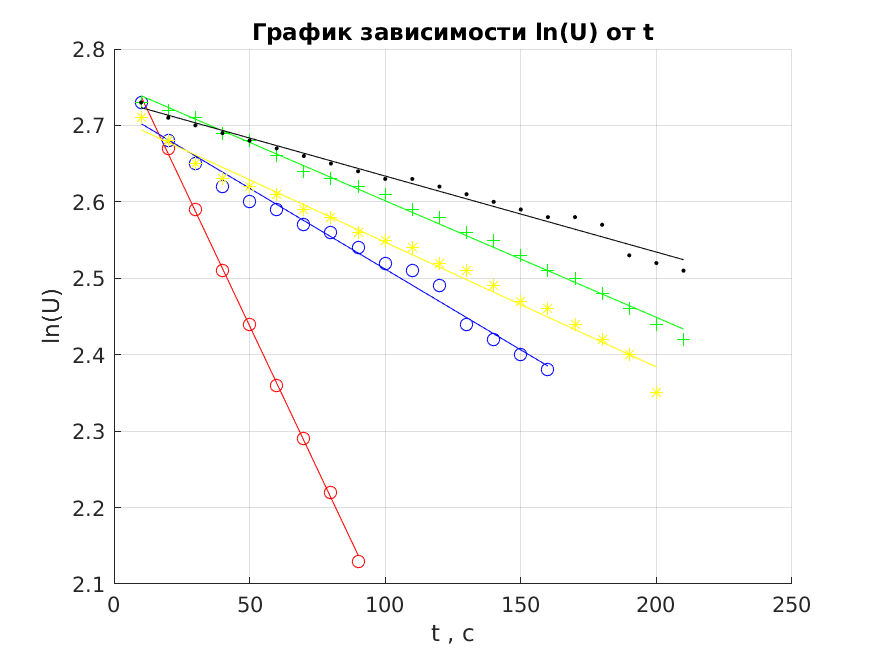
\includegraphics[scale = 0.68]{graph_1.png}}
\end{figure}

\newpage

\begin{figure}[h]
	\center{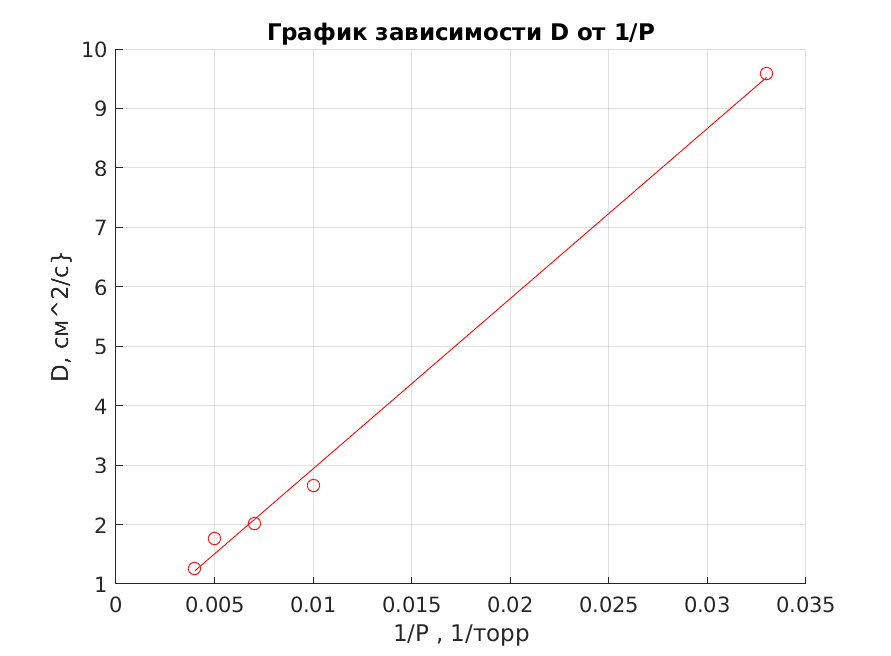
\includegraphics[scale = 0.68]{graph_2.png}}
\end{figure}


\section{Список используемой литературы}
$\bullet$ Гладун А. Д. Лабораторный практикум по общей физике. Термодинамика и молекулярная физика\\
$\bullet$ \href{https://mipt.ru/education/chair/physics/S_II/lab/}{Описание лабораторных работ на кафедре общей физики МФТИ}

\newpage



\end{document}
